\documentclass{article}

\usepackage{Mathematics}
\usepackage{graphicx}
\usepackage{titlesec}
\usepackage{titletoc}
\pdftitle{Environmental Analysis and Ecology}

\renewcommand{\thepart}{\Large Week }
\titleformat{\part}{\LARGE\bfseries\color{black}}{\thepart}{0em}{}

% === TITLE ===
\title{\textbf{Environmental Analysis and Ecology \\ HSLU, Semester 4}}
\author{Matteo Frongillo}
\date{}

% === TEXT ===
\begin{document}

\maketitle
\tableofcontents
\pagebreak

\part{1}
\section{\todo}
\pph{Carrying capacity in general systems:}
The maximum level of output or performance that a system can sustain over time without experiencing degradation or failure.

Sensitivity analysis: sensitivity of a single parameter and how much it impacts

Scenario analysis: optimization of multiple parameters to minimize the resultant impact

\pph{Carrying capacity in population:}
Maximum population size of a species that an environment can sustain indefinitely, given the available resources and environmental conditions.

\part{2}
\section{Systems}
\subsection{Characteristics}
\begin{itemize}
    \item Input and Output
    \item Set of components
    \item Rules and relationships between components
    \item System's boundaries
\end{itemize}

\subsection{System's loops}
\subsubsection{Feedback loops}
Feedback loops are the system's response to changes\\
Two types of loops:
\begin{itemize}
    \item Positive feedback loops (Reinforcing): \\
    Causes systems to change further in same direction
    \item Negative feedback loops (Balancing): \\
    Causes systems to change in opposite direction from which it is moving
\end{itemize}

\subsubsection{System's responses}
\paragraph{Time delays}
Complex systems often show time delays between input of a feedback stimulus and the response to it \textbf{(oscillating graph)} \\
Ex: Population growth or global climate change 

\paragraph{Synergistic interaction}
System effects can be amplified through synergistic interaction

\subsection{Casual loop diagram (CLDs)}
CLDs are maps showing casual links with arrows from a cause to an effect and it allows the identification of polarity of feedback loops (positive or negative)

\subsection{Reference Behavior Pattern (RBP)}
\begin{figure}[h]
    \centering
    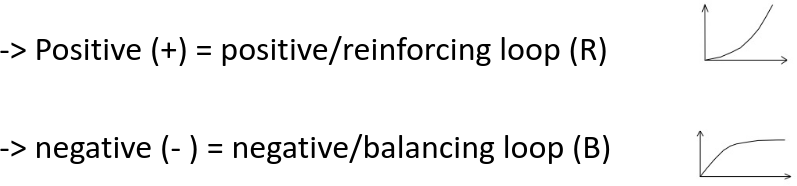
\includegraphics[width=0.8\textwidth]{media/feedbackloops.png}
    \caption{Reference Behavior Pattern}
\end{figure}

\paragraph{Example}
\begin{figure}[h]
    \centering
    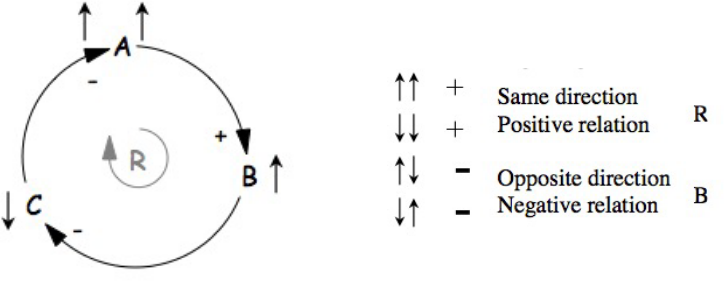
\includegraphics[width=0.8\textwidth]{media/feedbackloops2.png}
    \caption{RBP Example}
\end{figure}
If A increases, B will increase ($\uparrow\uparrow$)
\begin{itemize}
    \item Arrows show same direction $\rightarrow$ assign (-)
    \item Variables can also be decreasing in the same direction ($\downarrow\downarrow$) $\rightarrow$ also assign (-)
\end{itemize}

If B increases, C decreases ($\uparrow\downarrow$)
\begin{itemize}
    \item Arrows show opposite directions $\rightarrow$ assign (-)
\end{itemize}

If C decreases, A increases ($\downarrow\uparrow$)
\begin{itemize}
    \item Arrows show opposite directions $\rightarrow$ assign (-)
\end{itemize}

So:\\
A$\uparrow$ $\rightarrow$ B$\uparrow$ $\rightarrow$ C$\downarrow$ $\rightarrow$ A$\uparrow\uparrow$ (Reinforcing Loop) \\
A$\downarrow$ $\rightarrow$ B$\downarrow$ $\rightarrow$ C$\uparrow$ $\rightarrow$ A$\downarrow\downarrow$ (Reinforcing Loop)

\section{Ecosystems}
\subsection{Energy flow in ecosystems}
Robustness in ecosystems is the capacity of an ecosystem to withstand disturbances (e.g., drought, fire, pollution) while maintaining its structure and key functions.

It is important because it helps prevent collapse into degraded states and preserves ecosystem services like nutrient cycling, productivity, and biodiversity support.

\subsection{Cycles in the biosphere}
\subsubsection{Nutrient cycle}
\todo

\subsubsection{Hydrologic cycle}
\todo

\subsubsection{Nitrogen cycle}
\begin{itemize}
    \item Major reservoir for the nitrogen is the atmosphere (78\%)
    \item Nitrogen cannot be directly absorbed and used as a nutrient by plants or animals
\end{itemize}

\paragraph{Human alteration}
\begin{itemize}
    \item Humans add large amounts of nitric oxide (NO) into the atmosphere by burning any fuel at high temperatures (e.g. car, jet engines) $\rightarrow$ acid rain
    \item Nitrous oxide (N$_2$O) in atmosphere through commercial inorganic fertilizers $\rightarrow$ N$_2$O is a GHG and depletes stratospheric ozone
    \item Large quantities of nitrogen stored in soils and plants through destruction of forests, grasslands, and wetlands
    \item Humans alter nitrogen cycle in aquatic ecosystems through agricultural runoff and discharges from municipal sewage systems
\end{itemize}

\subsubsection{Phosphorus cycle}
\begin{itemize}
    \item Phosphorus circulates in the soil mainly, also through water, the earth's crust, and living organisms
    \item As water runs over exposed phosphorus-containing rocks and dissolves phosphate
    \item Phosphate is mainly absorbed by plants roots
\end{itemize}

\paragraph{Human alteration}
\begin{itemize}
    \item Removal of large amounts of phosphate from the earth to make fertilizers
    \item Soil from fertilized crop fields carries large quantities of phosphates into streams, lakes and the ocean, where it stimulates the growth of algae
    \item Phosphate runoff from sewage water and mining waste
\end{itemize}

\subsubsection{Sulphur cycle}
\begin{itemize}
    \item Most of the earth’s sulphur is stored underground in rocks and minerals, including sulphate salts buried under ocean sediments
    \item Sulphur also enters the atmosphere from several natural sources (e.g. active volcanoes, organic matter, which is broken down by anaerobic decomposers) $\rightarrow$ Deposited as acid rain
\end{itemize}

\paragraph{Human alteration}
\begin{itemize}
    \item Release of large amounts of sulphur dioxide into the atmosphere $\rightarrow$ Acid rain
    \begin{itemize}
        \item Burning of coal and oil to produce electric power
        \item Refining of sulphur-containing fossil fuels to make gasoline and heating oil
        \item Conversion (smelting) sulphur-containing metallic mineral ores into free metals such as copper, lead, and zinc
    \end{itemize}
\end{itemize}

\subsubsection{Carbon cycle}
\begin{itemize}
    \item Carbon cycle is based on carbon dioxide (CO$_2$)
    \item 0.038\% of the atmosphere consists of CO$_2$
    \item CO$_2$ is a key component of nature’s thermostat:
    \begin{itemize}
        \item If too much CO$_2$ is removed from the atmosphere $\rightarrow$ atmosphere gets cooler
        \item If too much CO$_2$ is added to the atmosphere $\rightarrow$ atmosphere gets warmer
    \end{itemize}
    \item Plants and animals exchange CO$_2$ with the atmosphere through photosynthesis and respiration
    \item Carbon stored more permanently in plants returns to atmosphere as CO$_2$ through decomposition
    \item Oceans absorb and emit carbon to the atmosphere, and some of this carbon ends up accumulated at the bottom of the ocean
    \item Humans heavily contribute carbon to the atmosphere:
    \begin{itemize}
        \item Extraction of fossil fuels $\rightarrow$ CO$_2$ emissions due to combustion
    \end{itemize}
\end{itemize}

\part{3}
\section{Biodiversity}
\subsection{Definition}
Biodiversity is the variety of earth͛s species, the genes they contain, the ecosystems in which they
live and the ecosystem processes (energy flow and nutrient cycling).

\todo

\section{Species diversity}
\subsection{Population dynamics}
\subsubsection{Population}
Group of individuals of the same species that live in the same place at the same time

\subsubsection{Population factors}
\begin{itemize}
    \item Distribution
    \item Size
    \item Age structure
    \item Density
\end{itemize}

\subsubsection{Population dynamics}
Study of how population characteristics change in response to changes in environmental
conditions.

Four factors that determine population size:
\begin{itemize}
    \item Births
    \item Deaths
    \item Immigration
    \item Emigration
\end{itemize}

Population change is defined as:
\figbox{population change = (births + immigration) - (deaths + emigration)}

Age structure can have a strong effect on how rapidly a population size increases or decreases:
\begin{itemize}
    \item Pre-reproductive age (not mature enough to reproduce)
    \item Reproductive stage (capable of reproduction)
    \item Post-reproductive stage (too old to reproduce)
\end{itemize}

\subsubsection{Growth functions}
Species vary in their capacity for population growth under ideal conditions

\subsubsection{Intrinsic rate of increase}
Rate at which the population of a species would grow if it had unlimited resources.

Populations with high intrinsic rate of growth typically reproduce early in life, have short
generation times (time between successive generations), can reproduce many times, and have
many offspring each time they reproduce.

\subsubsection{Carrying capacity}
Intrinsic rate of increase and environmental resistance = carrying capacity.

\pph{Definition:}
Maximum population of a given species that a particular habitat/area can sustain
indefinitely without being degraded

\begin{itemize}
    \item Carrying capacity of an area is not fixed
    \item A population with few (or no) limitations can grow exponentially
    \item Environmental resistance slows down growth rate as population size gets closer to carrying capacity:\\\textrightarrow\ logistic growth curve or S-shaped growth curve
\end{itemize}

\subsection{Human influence}
Extinction rate caused by human influence will increase to 10,000 times the
background extinction within this century.

Annual extinction rate of ca. 1\% per year (currently between 0.01 - 0.1\%)

New species eventually evolve to take the places of the lost one.

\part{4}
\section{Stock and flow diagrams (SFD)}
\subsection{Translating CLDs into SFDs}
\begin{itemize}
    \item CLDs represent conceptual models, which depict causal mechanisms based on underlying reference behaviour patterns (RBPs)
    \item First step in computational modelling of CLDs is the translation of CLDs into SFDs
\end{itemize}

\subsection{Stock and flow diagrams (SFDs)}
\begin{itemize}
    \item SFDs provide a richer visual language than CLDs
    \item Six basic elements exist in SFDs: \textbf{Stocks, Flows, Converters, Connectors, Sources, and Sinks}
\end{itemize}

\subsection{Components of SFDs}
\subsubsection{Stocks}
A stock is a ``part of a system whose value at any given instant in time depends on the systems past behavior''.

A stock is defided as:
\figbox{Stock = $\integral[t_0][t_1][\text{(inflow - outflow)}][t] + \text{value right before starting}$}

\begin{itemize}
    \item Stocks represent anything that accumulates (normally in both directions)
    \item \textbf{Stocks are only affected by inflows and outflows}
    \item Stocks are normally tangible, countable and physical
    \begin{itemize}
        \item But can also be non-physical (e.g. level of fear, aggression)
        \item Non-tangible stocks require special attention, since differences in numerical translation might cause different system behaviours
    \end{itemize}
    \item Stocks are usually presented by nouns
\end{itemize}

\subsubsection{Flows}
\begin{itemize}
    \item Represent activities that lead to inflows and outflows to stocks (e.g. births, migration)
    \item Inflows cause the stock to increase
    \item Outflows decrease the stock
    \item Flows are usually presented by verbs or nouns describing an action
\end{itemize}

\begin{center}
    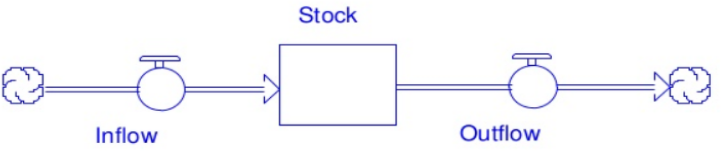
\includegraphics[width=0.55\textwidth]{media/flows_stella.png}
\end{center}

\begin{minipage}{0.5\textwidth}
    \subsubsection{Converter}
    \begin{itemize}
        \item Contain equations that generate an output value during each time interval of a simulation\\(e.g. birth rate, migration rate)
        \item Can also be used for storing constant values\\(e.g. initial population size)
    \end{itemize}

    \subsubsection{Connectors}
    \begin{itemize}
        \item Transmit information to regulate flows
        \item Connectors can connect into flows or converters but never into stocks
    \end{itemize}
\end{minipage}
\hfill
\begin{minipage}{0.45\textwidth}
    \centering
    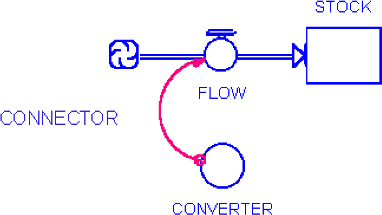
\includegraphics[width=\textwidth]{media/connectors_stella.png}
\end{minipage}

\subsubsection{Source and Sink}
\begin{itemize}
    \item Stocks that lie outside the system boundary
    \item Sources and sinks are shown as clouds in the diagram.
    \item Are used to show that a certain stock inflow is coming from another source (e.g. migration)
    \item Or that an outflow ends up in another stock outside the system (e.g. emigration)
\end{itemize}

\begin{center}
    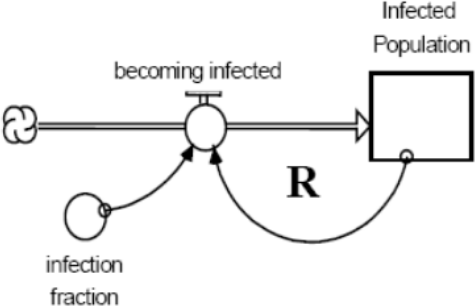
\includegraphics[width=0.4\textwidth]{media/sinks.png}
\end{center}

\newpage
\part{5}
\section{Climate}
\subsection{Weather vs. climate}
Weather:
\begin{itemize}
    \item Weather is a local, short term phenomenon
    \item Weather is mainly expressed by temperature, humidity, precipitation, wind speed, cloud cover
    \item Measured over hours or days
\end{itemize}

Climate:
\begin{itemize}
    \item Area’s general pattern of atmospheric or weather conditions
    \item Measured over long periods of time (ranging from decades to thousands of years)
\end{itemize}

\subsection{Climate factors}
\subsubsection{Climate zones}
\begin{itemize}
    \item Important component of earth's natural capital
    \item Climate variations caused by patterns of global air circulation and ocean currents
\end{itemize}

\subsubsection{Factors of air circulation in lower atmosphere}
\begin{minipage}{0.5\textwidth}
    \begin{itemize}
        \item Uneven heating of earth's surface $\to$\ Air is heated more at the equator
        \item Rotation of the earth around its axis:
        \begin{itemize}
            \item Heated air masses rise above equator and move north and south
            \item Atmosphere divided in cells, distinguished by direction of air movement
            \item Differing directions of air movement are called \textbf{prevailing winds} (major surface winds that blow almost continuously and distribute air, heat, moisture and dust)
            \item Prevailing winds also produce mass movements of surface water (currents)
        \end{itemize}
        \item Properties of air, water and land:
        \begin{itemize}
            \item Heat from the sun evaporates ocean water and transfers heat from the oceans to the atmosphere, especially near the equator
            \item Evaporation of water creates cells (low and high pressure) which circulate air, heat, and moisture
        \end{itemize}
    \end{itemize}
\end{minipage}
\hfill
\begin{minipage}{0.45\textwidth}
    \centering
    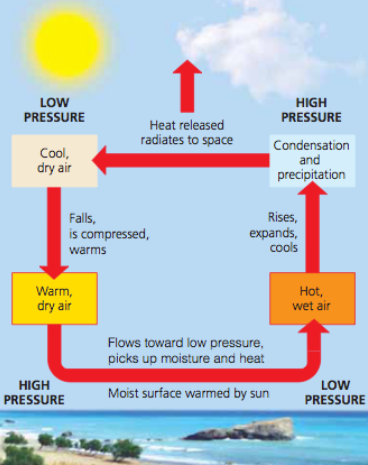
\includegraphics[width=\textwidth]{media/climate_pressure.png}
\end{minipage}

\subsubsection{Ocean conveyer belt (thermohaline circulation)}
\begin{itemize}
    \item Heat is also distributed when ocean water mixes vertically in shallow and deep ocean currents
    \item Result of differences in the seawater density
    \item Colder seawater (higher density) sinks and flows beneath warmer and less dense seawater
    \item Connected loop of deep and shallow ocean currents
    \item Acts like giant conveyer belt that moves heat to and from the deep sea
    \item Transfers warm and cold water between tropics and poles
\end{itemize}

\subsubsection{Link between ocean and atmosphere}
\begin{itemize}
    \item Ocean currents are affected by winds in the atmosphere
    \item Heat from the ocean affects atmospheric circulation
\end{itemize}

\subsubsection{Earth's surface features}
\begin{itemize}
    \item Heat is absorbed and released more slowly by water than by land:\\
    $\to$\ Difference creates land and sea breezes $\to$\ oceans and large lakes moderate weather and climates of nearby lands
    \item Topographic features of earth’s surface can create local and regional weather and climatic conditions that differ from the general climate of a region (e.g. mountains)
\end{itemize}

\subsubsection{Greenhouse effect warms lower atmosphere}
\begin{itemize}
    \item Greenhouse gases allow visible light (and some infrared radiation and UV radiation) from the sun to pass through the atmosphere
    \item Earth’s surface absorbs much of this solar energy and transforms it to heat, which then rises into the lower atmosphere
    \item Some of this heat escapes into space, but some is absorbed by molecules of greenhouse gases $\to$\ Warms the lower atmosphere and the earth’s surface (greenhouse effect)
\end{itemize}

\section{Climate change - natural cycles}
\subsection{Characteristics of climate change}
\subsubsection{Natural variations}
\begin{itemize}
    \item Changes of earth’s climate are neither new nor unusual
    \item Atmosphere has experienced prolonged periods of global cooling and global warming
    \item Alternating cycles of cooling and warming are called glacial and interglacial periods
\end{itemize}

\section{Natural forces}
\subsection{Milankovitch cycle}
\subsubsection{Variations}
\pph{Earth's orbit}
Earth’s orbit changes from being nearly circular to slightly elliptical (termed ‘eccentricity’)
\begin{itemize}[label=$\to$]
    \item Cycle has a period of around 100.000 years
    \item The more elliptic the orbit becomes, the less time the earth spends near the sun
    \item Less solar energy leads to cooling effect
\end{itemize}

\pph{Angle of tilt}
Angle of tilt of the earth’s axis changes from 22,1$^\circ$ (22,5) to 24,5$^\circ$ (term ‘obliquity’)
\begin{itemize}[label=$\to$]
    \item Cycle has a period of 41.000 years
    \item Land mass of the northern hemisphere face more/less towards the sun
    \item Leads to cooling/warming effects
\end{itemize}

\pph{Direction of tilt}
Direction of tilt of the axis changes (termed ‘precession’)
\begin{itemize}[label=$\to$]
    \item Cycle has a period of 26.000 years
    \item Causes winters and summers to be warmer or colder depending on the amount of land surface being more or less exposed to the sun
\end{itemize}

\section{Anthropogenic climate change}
\subsection{Global warming}
\subsubsection{Today's climate}
\begin{itemize}
    \item For ca. 10,000 years earth’s climate is in an interglacial period
    \item It is characterized by a fairly stable climate and a fairly steady average global surface temperature\\$\to$\ Allows agriculture $\to$\ triggered population growth
    \item Average temperature of the atmosphere has remained fairly stable for the last 1,000 years
    \item Temperature started rising during last century
\end{itemize}
\vspace*{.2cm}
\begin{center}
    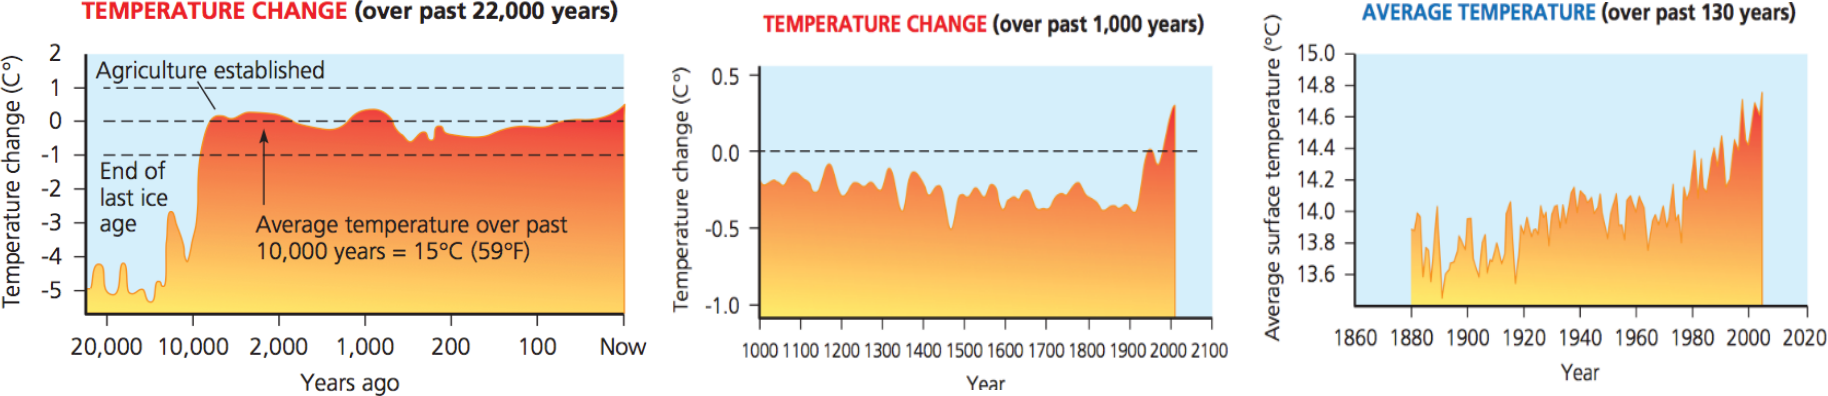
\includegraphics[width=\textwidth]{media/temperature_change.png}
\end{center}

The 0 temperature change line was set based of the average temperature
right after the beginning of the industrial revolution.

\subsection{Greenhouse effect}
\begin{itemize}
    \item Life depends on natural greenhouse effect $\to$\ Without natural greenhouse effect no life would exist and earth would be too cold
    \item Since Industrial Revolution significant increase in CO$_2$, CH$_4$, and N$_2$O concentration in lower atmosphere $\to$\ Increases is mainly due to agriculture, deforestation and burning of fossil fuels
    \item Measurements of CO$_2$ and CH$_4$ in glacial ice cores indicate high correlation between concentration level and average global temperature
\end{itemize}

\subsection{Greenhouse gas emission}
\begin{itemize}
    \item CO$_2$ level has risen from 280 ppm (around 275 years ago) to 399 ppm in 2014
    \item If CO$_2$ emissions continue to increase at current rate of about 3.3\% a year
    \begin{itemize}[label=$\to$]
        \item Levels will rise to 560 ppm by 2050 and to 1,390 ppm by 2100
        \item Significant changes in earth’s climate
        \item Major ecological and economic disruptions
    \end{itemize}
    \item CO$_2$ levels should be prevented from exceeding 450 ppm\\
    $\to$\ Estimated tipping point that sets into motion large-scale climate changes
    \item Ideally: reduction of CO$_2$ to 350 ppm (pre-industrial level)\\
    $\to$\ Stabilizing earth’s climate
\end{itemize}

\subsubsection{CO$_2$ emission over time}
\begin{center}
    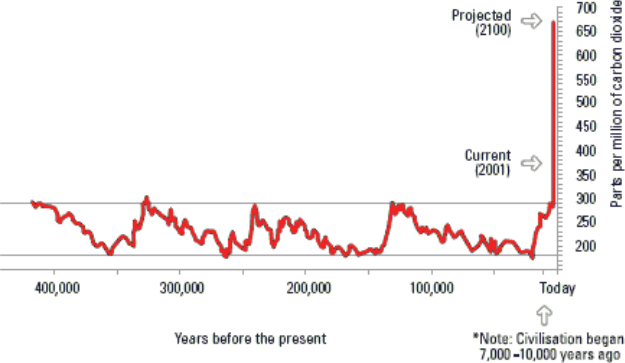
\includegraphics[width=.6\textwidth]{media/greenhouse_gas_emission.png}
\end{center}

Due to the periodic changes in the Earth's orbit, from elliptical to
circular and vice versa, the more elliptical the orbit is, the
farther the Earth is from the Sun, the fewer plants there are, and
the less CO$_2$ is stored.

Nowadays, the amount of CO$_2$ in the atmosphere is higher than ever
due to industrialization.

\subsubsection{Global Warming Potential (GWP)}
\begin{itemize}
    \item Describes potential impact of each greenhouse gas (GHG)
    \item Some GHGs are more effective at warming the atmosphere than others
    \item Most important characteristics of a GHG in terms of climate impact are:
    \begin{itemize}[label=$\to$]
        \item Energy absorption potential (preventing energy from escaping to space)
        \item Residence time of gas in atmosphere
    \end{itemize}
    \item GWP measures total energy that gas absorbs over 100 years, compared to CO$_2$
\end{itemize}

\vspace*{.2cm}
\begin{center}
    {\renewcommand{\arraystretch}{2}
    \begin{tabular}{lccc}
        \hline Greenhouse Gase & \makecell{Chemical\\formula} & \makecell{Global Waeming\\20 years} & \makecell{Potential {\small (Time horizon)}\\100 years}\\
        \hline Carbon dioxide & CO$_2$ & 1 & 1\\
        \hline Methane & CH$_4$ & 42-70 & 16-26\\
        \hline Nitrous oxide & N$_2$O & 280$\quad$ \tikzmark{a} & \tikzmark{b}$\quad$310 \\
        \hline 
    \end{tabular}}
    \begin{tikzpicture}[overlay,remember picture]
        \draw[<->,thick] ([yshift=1ex]pic cs:a) -- ([yshift=1ex]pic cs:b);
    \end{tikzpicture}
\end{center}

\subsubsection{Methane CH$_4$}
\begin{itemize}
    \item 60\% of methane emissions occurred during last 275 years
    \item Extraction of fossil fuels, creating landfills, raising cattle and sheep
    \item CH$_4$ emissions have levelled off since 1990
    \item Are expected to rise again $\to$\ melting of permafrost in the arctic tundra
    \item GWP: 16-26 times greater than CO$_2$
\end{itemize}

\subsubsection{Nitrodus oxide N$_2$O}
\begin{itemize}
    \item Nitrous oxide levels have risen ca. 20\% during last 275 years
    \item Increased use of nitrogen fertilizers
    \item GWP: 280 times greater than CO$_2$
\end{itemize}

\subsection{Effects of a warmer atmosphere}
\subsubsection{Extreme weather events}
\begin{itemize}
    \item Increased incidence of extreme weather events such as heat waves, droughts, flooding
    \item Controversy over the question if global warming also increases frequency and intensity of tropical storms and hurricanes
    \item Hurricane Katrina caused loss of over 320 million big trees\\
    $\to$\ dead and damaged trees emitted CO$_2$ equal to the total amount that all forest trees in the U.S. absorb in one year
\end{itemize}

\subsubsection{Effects on biodiversity}
\begin{itemize}
    \item ca. 30\% of the land-based plant and animal species could disappear if average global temperature change exceeds 1.5-2.5 $^\circ$C
    \item Percentage could grow to 7\% if temperature change exceeds 3.5 $^\circ$C
    \item Hardest hit will be plant and animal species in colder climates
    \item Global warming could also disrupt biological clocks of birds, whales, and other migratory species
    \item Ecosystems will suffer disruption (e.g. coral reefs, polar seas) $\to$\ species extinction
\end{itemize}

\subsubsection{Effects on humans}
\pph{Nutrition}
\vspace*{-.4cm}
\begin{itemize}
    \item Agricultural productivity may increase in some areas and decrease in others
    \item Crop productivity is projected to increase slightly at middle to high latitudes
    \item Agricultural productivity will decrease in tropical and subtropical regions
    \item Flooding of rivers and droughts reduces crop production
    \item IPCC warns that ca. 200-600 million people could face malnutrition/starvation from climate change effects
\end{itemize}

\pph{Health}
\vspace*{-.4cm}
\begin{itemize}
    \item Fewer people will die from cold weather, but heat-related deaths will increase
    \item Better living conditions for rapidly multiplying insects, microbes, toxic moulds
    \item Infectious diseases (e.g. dengue fever, yellow fever, malaria) are likely to expand their ranges
    \item Higher atmospheric temperatures also increases some forms of air pollution\\
    $\to$\ Speeds up chemical reactions, which causes photochemical smog in urban areas
    \item WHO estimates that currently each year, climate change contributes to premature deaths of more than 150'000 people
\end{itemize}

\subsubsection{Reduction of GHG emissions}
\pph{4 steps for CO$_2$ reduction}
\vspace*{-.4cm}
\figbox{\begin{enumerate}[label=\textbf{\arabic*.}]
    \item Change the type of fuel (conversion of primary source)
    \item Maximize the efficiency of conversion of the fuels
    \item Increase the energy efficiency of the device itself
    \item Change the behavior of the humans
\end{enumerate}}

\pph{Major GHG reduction strategies}
\vspace*{-.4cm}
\begin{itemize}
    \item Improving energy efficiency to reduce fossil fuel use
    \item Shift from non-renewable (carbon-based) fuels to (carbon-free) renewable energy sources
    \item Stop cutting down tropical forests
    \item Effectiveness of these strategies would be enhanced by reducing population\\
    \begin{itemize}[label=$\to$]
        \item Decreasing number of CO$_2$ emitters
        \item Reducing poverty
        \item Decreasing need to clear more land for crops and fuel wood
    \end{itemize}
\end{itemize}

\pph{Geo-engineering}
\vspace*{-.4cm}
\begin{itemize}
    \item Capturing and storage of CO$_2$ (and keep burning fossil fuels)
    \item Injection of sulphate particles into stratosphere $\to$\ reflection of incoming sunlight
    \item Space sunshades
\end{itemize}

\part{6}
\section{Analytical tools for energy and environmental systems}
\subsection{Characteristics of energy systems}
\subsubsection{Relationship between energy use and wealth}
\begin{itemize}
    \item Most used measure for wealth = GDP
    \item GDP = sum of monetary value of all goods and services produced in a country/year
    \item GDP value may be adjusted to reflect purchasing power parity (PPP) $\to$\ A dollar equivalent earned in one country may not buy as much as in another country
    \item GDP per capita is correlated with energy use per capita $\to$\ GDP rises with energy use (per capita)
\end{itemize}

\subsubsection{Quality criteria of energy resources}
\begin{itemize}
    \item Must be reliable and deliver the service that the consumer expects
    \item Must be available in the quantity desired and when the consumer wishes to consume it
    \item Resource must be available at a price that is economically affordable
    \item If quality criteria are not met, direct consequences are experienced
\end{itemize}

\subsubsection{Long term criterion}
\begin{itemize}
    \item Another criterion for energy resource is environmental sustainability
    \item Problem: consumers of energy resources do not experience direct consequences if this criterion is not met
\end{itemize}

\subsection{Energy systems categories}
\begin{itemize}
    \item Physical goals
    \item Financial goals
    \item Environmental goals
\end{itemize}

\subsubsection{Physical goals}
\begin{itemize}
    \item Physical requirements that make it possible for the system to operate
    \item All systems require primary energy resources
    \item Any type of energy system must function efficiently, reliably, and safely
\end{itemize}

\subsubsection{Financial goals}
\begin{itemize}
    \item For small-scale, privately held systems goal might be to reduce energy
    \item For commercial energy systems the goal is normally profit maximisation (returning profits to shareholders)
\end{itemize}

\subsubsection{Environmental goals}
\begin{itemize}
    \item Reduction of GHG emissions
    \item Reduction of air pollutants $\to$\ increase of air quality
    \item Minimization of physical effects from extracting resources
    \item Minimization of impacts on physical surroundings, such as noise or vibrations
    \item Reduction of (thermal) pollution of water
    \item Avoidance of disruption of natural habitats
\end{itemize}

\subsection{Objectives}
\begin{itemize}
    \item Use of existing technology options in a different way
    \item Conserving energy by replacing end-use technology $\to$\ Primary energy source remains the same, but new technology is introduced to use energy resource more efficiently
    \item Conserving energy by replacing conversion technology $\to$\ Same primary source of energy (e.g., fossil fuels), but conserve energy by replacing the energy conversion device with a more efficient model
    \item Replacing existing energy sources with alternatives
\end{itemize}

\subsubsection{Overall sustainability objectives (Sustainable development)}
\begin{itemize}
    \item Environmental sustainability: protection of the environment
    \item Social/cultural sustainability: increasing equity (decreasing poverty)
    \item Economic sustainability: responsible economic development
\end{itemize}

\begin{center}
    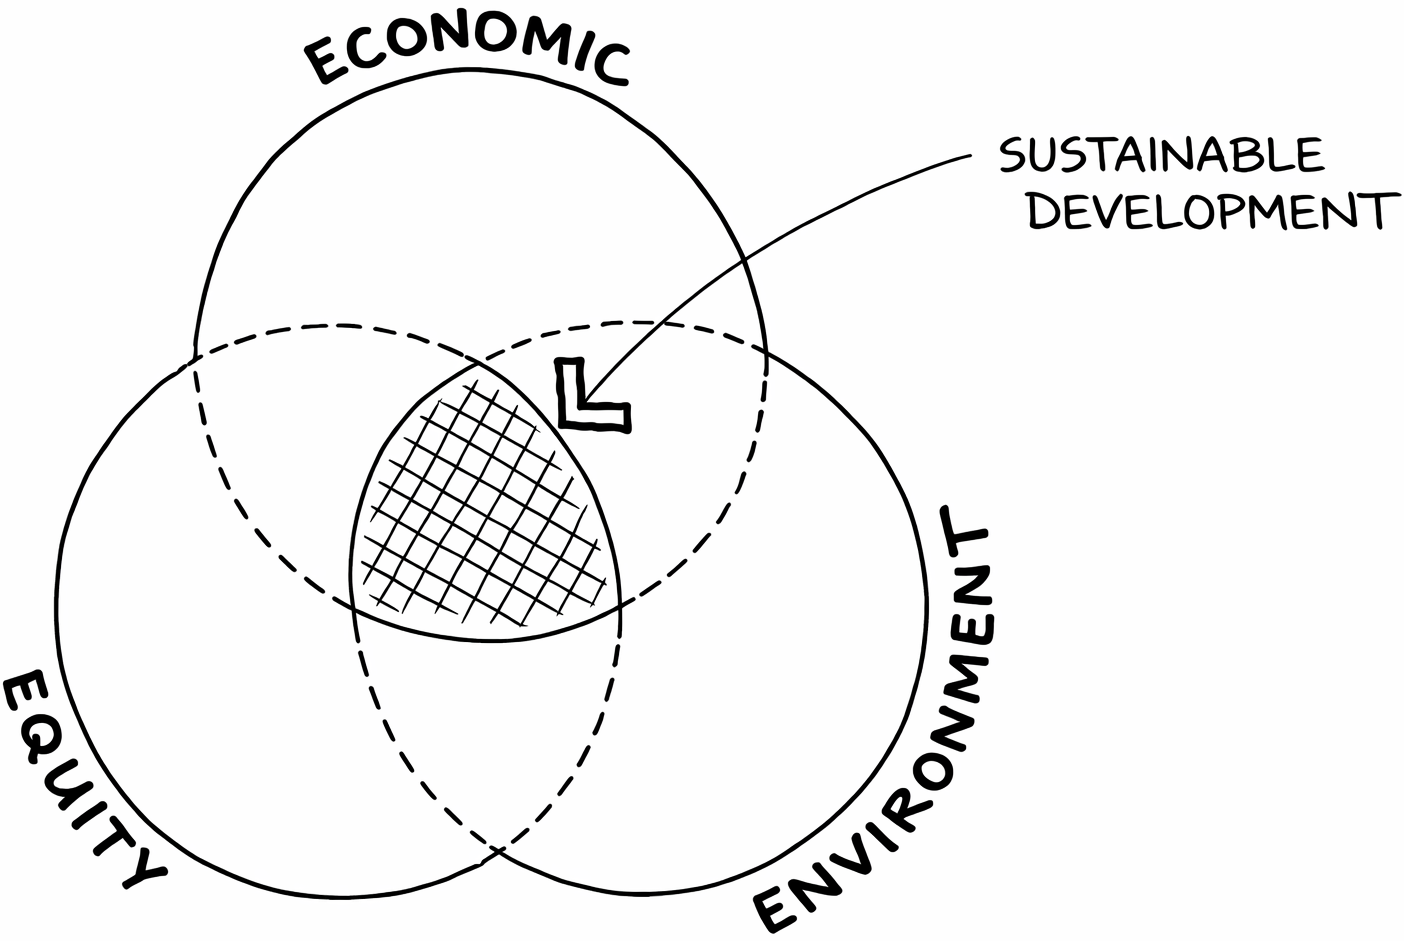
\includegraphics[width=.4\textwidth]{media/sustainable_development.png}
\end{center}

\subsection{Definition of energy systems}
\begin{itemize}
    \item ``A system is a set of components that function and interact in some regular way''
    \item Group of interacting components that work together to achieve some common purpose
    \item Each system has a boundary: physical or conceptual $\to$\ Entities or objects that are not part of system lie outside the boundary
    \item Area outside the boundary is called the environment
    \item Energy systems have input and output flow between the system and its environment
    \item Inputs and outputs may be physical (e.g. raw materials) or virtual (e.g. information, data)
    \item Systems can consist of subsystem (e.g. electricity grid)
    \item Defining boundaries, input and output flows and subsystems is essential
\end{itemize}

\subsubsection{Energy systems diagram}
\begin{center}
    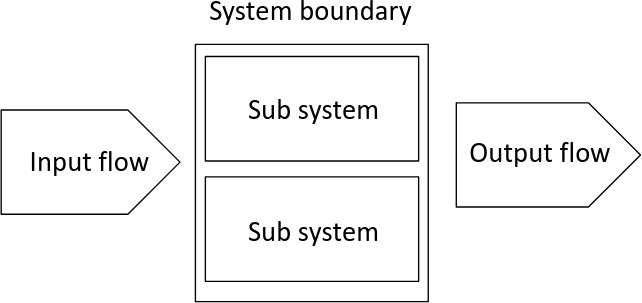
\includegraphics[width=.6\textwidth]{media/energy_systems.png}
\end{center}

where:
\begin{itemize}
    \item \textbf{System boundary}: defines what is included in the analysis and what is outside the system to study the relevant components and interactions
    \item \textbf{Input flow}: represents the resources entering the system, such as energy, materials, or information
    \item \textbf{Sub system}: a smaller internal part of the main system with a specific function
    \item \textbf{Output flow}: represents what leaves the system, such as useful energy, waste, emissions, or information
\end{itemize}

\subsection{Energy return on investment (EROI)}
\begin{itemize}
    \item End-use energy derived from a particular resource needs to justify energy expended upstream in its extraction, conversion and delivery:
    \begin{itemize}
        \item \textbf{Upstream: everything before the operational phase}
        \item \textbf{Downstream: energy or money used to dismantle the energy system or to end it}
    \end{itemize}
    \item EROI = energy delivered at the end of the life cycle / energy used in earlier stages
    \item EROI presents the amount of energy returned from the use of an energy source after expending energy on manufacture, installation etc.
\end{itemize}

\subsection{Energy payback time (EPBT)}
\begin{itemize}
    \item EPBT expresses the years it takes for a certain technology to produce as much net energy as it takes to manufacture and dispose the technology
    \item Used as a measure of energy efficiency from an investment perspective
    \item EPBT must be much less than lifetime of technology
\end{itemize}

\figbox{\centering $\dm \text{EPBT} = \frac{\text{Cumulative energy demand}}{\text{Yearly net energy generated}}$\\[2ex]
        $\dm \text{EPBT} = \frac{E_\text{Materials} + E_\text{Manufactoring} + E_\text{Installation} + E_\text{Disposal recycling}}{\text{Energy generated} - E_{\text{O\&M}}}$}

where $E_\text{O\&M}$ is the energy used in operations and maintenance, which is subtracted from the energy generated


\subsection{Kaya equation (Kaya identity)}
\begin{itemize}
    \item System approach for analysing factors that contribute to overall CO$_2$ emissions (country or global base)
    \item Approach includes population, level of economic activity, level of energy consumption, and carbon intensity
\end{itemize}

\figbox{$\dm CO_2 = P\cdot \frac{GDP}{P}\cdot \frac{E}{GDP}\cdot \frac{CO_2}{E}$}

where:
\begin{itemize}
    \item $P$: population (of a specific country)
    \item $GDP/P$: production per capita (to evaluate how wealthy the population is)
    \item $E/GDP$: energy intensity per unit of GDP (energy intensity of the population's economy / how much energy do you need to produce \$1)
    \item $CO_2/E$: carbon emissions per unit of consumed energy
\end{itemize}

\part{7}
\section{Life Cycle Assessment (LCA)}
LCA is an analytical tool that assesses energy consumption/emissions
within a life cycle of a system (e.g. product, energy system, material).

\pph{Example: LCA of a reusable water bottle}
1. Crude oil extraction, 2. Transportation, 3. Refinery, 4. Manufactory/Assembly, 5. Transportation to consumption, 6. Use, 7. Disposal

\subsection{Precision vs. Accuracy}

\subsubsection{Precision}
Precision describes how close repeated measurements are to each other.
A method is precise when it produces very similar results under the
same conditions.

\subsubsection{Accuracy}
Accuracy describes how close a measurement is to the true or accepted
value. Accuracy is only meaningful when the result is also sufficiently
precise, because a correct value obtained by chance is not reliable.

\subsection{Four phases of LCA}
\begin{minipage}{.55\textwidth}
    \renewcommand{\baselinestretch}{1.5}\selectfont
    \begin{enumerate}[label=\textbf{\arabic*}.]
        \item Goal and scope definition
        \item Inventory Analysis (LCI): compiling relevant inputs and outputs
        \item Impact Assessment (LCIA): evaluating potential environmental impacts associated with the inputs and outputs
        \item Interpretation: evaluation of results (LCI and LCIA) in relation to objectives of LCA
    \end{enumerate}
\end{minipage}
\hfill
\begin{minipage}{.37\textwidth}
    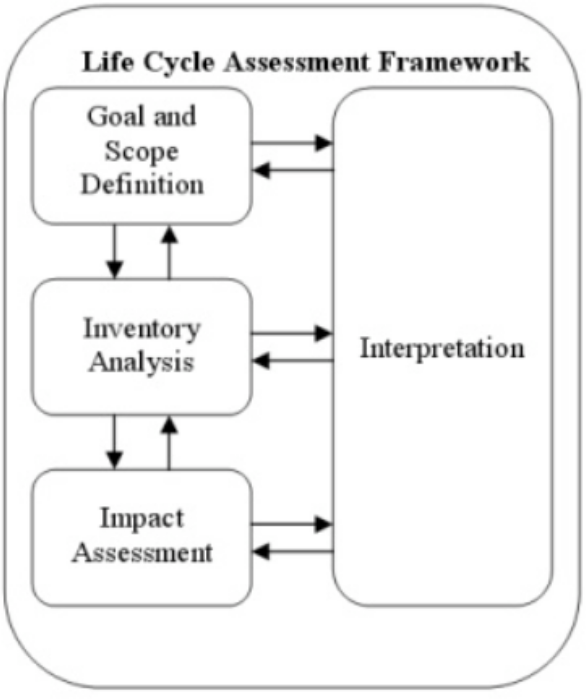
\includegraphics[width=\linewidth]{media/LCA.png}
\end{minipage}

\subsubsection{Goal and scope definition}
\begin{itemize}
    \item \underline{\textbf{Breadth and depth of the study is defined}}
    \item Goal should include statement of the reason for carrying out the LCA
    \item Scope should include the following:
    \begin{itemize}
        \item Function of the considered system
        \item Check for fixed bias (a measurement tool that gives you always the same fixed error)
        \item System boundaries (including assumptions and limitations)
        \item Data requirements
        \item Type of impact assessment methodology (LCIA)
    \end{itemize}
    \item Funcional unit:
    \begin{itemize}
        \item \underline{\textbf{It is needed to normalize the output so that can be compared with other outputs}}\\ \underline{\textbf{with the same functional unit}}
        \item Provides reference to which the inputs and outputs (inventory analysis) can be related to
        \item Enables possibilities for comparison between different systems
    \end{itemize}
\end{itemize}

\pph{Tools for analysing energy systems}
\vspace*{-.4cm}
\begin{itemize}
    \item Requires estimate of in- and outflow values for each stage of the life cycle
    \item It is partly very difficult to accurately estimate these values for each activity (e.g. energy consumed in individual stage)
    \item If no educated guess can be made, stage must be explicitly excluded from the LCA
    \item LCA can be performed from ``cradle to grave'' $\to$\ From resource extraction to disposal phase
    \item Or from ``cradle to cradle'' $\to$\ End-of-life disposal step for product is a recycling process
\end{itemize}

\subsubsection{Life cycle inventory analysis (LCI)}
\begin{itemize}
    \item \underline{\textbf{Collection of the input data}}
    \item Accounting of all processes involved in the system of interest
    \item Determination and quantification of all in- and outflows of the system:
    \begin{itemize}[label=$\to$]
        \item Raw resources or materials
        \item Types and amount of energy
        \item Water use
        \item Emissions to air, water and land by specific substance
    \end{itemize}
\end{itemize}

\pph{Overview of different stages within life cycle}
\begin{table*}[ht!]
    \renewcommand{\baselinestretch}{1.5}\selectfont
    \begin{tabular}{lll}
        Resource extraction & Transportation raw material & Conversion of raw material\\
        Product manufacturing & Product transportation & Commercial ``overhead''\\
        \makecell[l]{Infrastructure construction\\[-1ex] and maintenance} & Product use phase / consumption & Demolition / disposal / recycling\\
    \end{tabular}
\end{table*}

\newpage
\subsubsection{Life cycle impact assessment (LCIA)}
\underline{\textbf{Evaluation of magnitude and significance of potential environmental impacts}}.

\pph{Classification and characterization}
\vspace*{-.4cm}
\begin{itemize}
    \item Selection of relevant impact categories (based on goal an scope)
    \item Impact potentials are calculated
\end{itemize}

\pph{Normalization and weighting}
\vspace*{-.4cm}
\begin{itemize}
    \item Both steps are voluntary according to ISO standard (ISO 14040)
    \item Normalization provides basis for comparing different types of environmental impact categories (same unit is assigned)
    \item Weighting assigns a weighting factor to each impact category depending on relative importance
\end{itemize}

\pph{LCIA - Impact categories (ICs)}
\vspace*{-.4cm}
\begin{itemize}
    \item ICs represent environmental issues of concern
    \item LCI results are assigned to various ICs
    \item Possible ICs:\\
    Global warming / climate change, Acidification, Smog formation, Stratospheric ozone depletion, Eutrophication, Human carcinogenicity, Ecotoxicity (aquatic, terrestial)
\end{itemize}

\subsection{Interpretation: Eco-indicator 99}
Eco-indicator assesses seriousness of three damage categories:
\begin{enumerate}
    \item \textbf{Damage to human health}:
    \begin{itemize}[label=$\to$]
        \item Expressed as the number of years life lost and the number of years lived disabled
        \item Combined as Disability Adjusted Life Years (DALYs)
    \end{itemize}
    \item \textbf{Damage to ecosystem quality}:
    \begin{itemize}[label=$\to$]
        \item Expressed as loss of species over a certain area during a certain time (using for instance CO$_2$e)
    \end{itemize}
    \item \textbf{Damage to resources}:
    \begin{itemize}[label=$\to$]
        \item Expressed as surplus energy needed for future extractions of fossil fuels and minerals
    \end{itemize}
\end{enumerate}

\subsubsection{Damage model for resources}
\begin{itemize}
    \item Extracting minerals reduces quality of remaining resources $\to$\ High quality resources are extracted first (high ore grade)
    \item Damage to resources will be experienced by future generations $\to$\ More effort (energy) required to extract same amount of resources; Expressed as ``surplus energy''
\end{itemize}

\subsubsection{Damage model for land-use (ecosystem quality)}
\begin{itemize}
    \item Mankind occupies large areas for urban and agricultural purposes $\to$\ Degradation of natural habitat; increased species extinction rate
    \item Different types of land-use have different effects
    \item Scale expresses decrease in species diversity per type of land use
\end{itemize}

\newpage
\subsubsection{Damage model for human health - emissions}
Subdivided in 4 steps:

\pph{Fate analysis}
\vspace*{-.4cm}
\begin{itemize}
    \item Chemical substances are released into the air, water and soil (compartments)
    \item Where substance will go and how long it remains there depends on properties of substance and compartment
    \item Fate analysis models transfer between compartments and degradation (lifetime) of substance (calculating concentrations in air and water)
\end{itemize}

\pph{Exposure}
Based on concentration levels, it is determined how much of a substance is actually consumed by living organisms.

\pph{Effect analysis}
Based on exposure level diseases and other harmful effects and there frequencies are predicted.

\pph{Damage analysis}
Predicted diseases are expressed as damage unit:
\begin{itemize}
    \item For humans expressed as DALY
    \item For toxic effects on ecosystems percentage of exposed plants and species is determined
    \item For acidification and eutrophication percentage of plants which is likely to disappear is determined
\end{itemize}

It is important to determine the correct scale of impact (locally or globally).

\part{8}
\section{LCA modelling}
\subsection{Product}
It is what serves the process, for instance plastic, metal, aluminum,
crude oil. The raw, virgin material is a product.

\subsection{Process}
A process creates the product. Whenever a product is transported,
refined, modelled, molded.

\section{Representative sampling for environmental QCQA}
QCQA = Quality Control and Quality Assurance

\begin{center}
    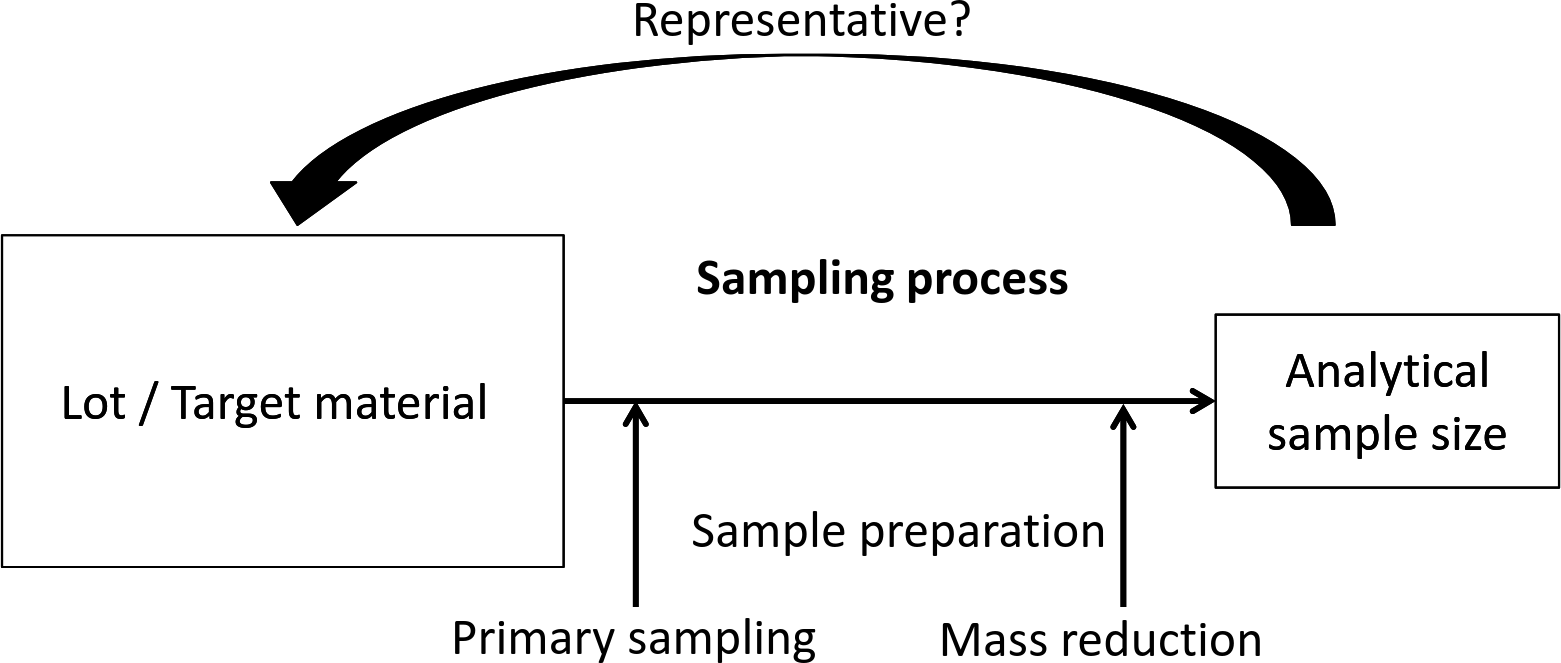
\includegraphics[width=.85\textwidth]{media/sampling.png}
\end{center}

\subsection{Material heterogeneity}
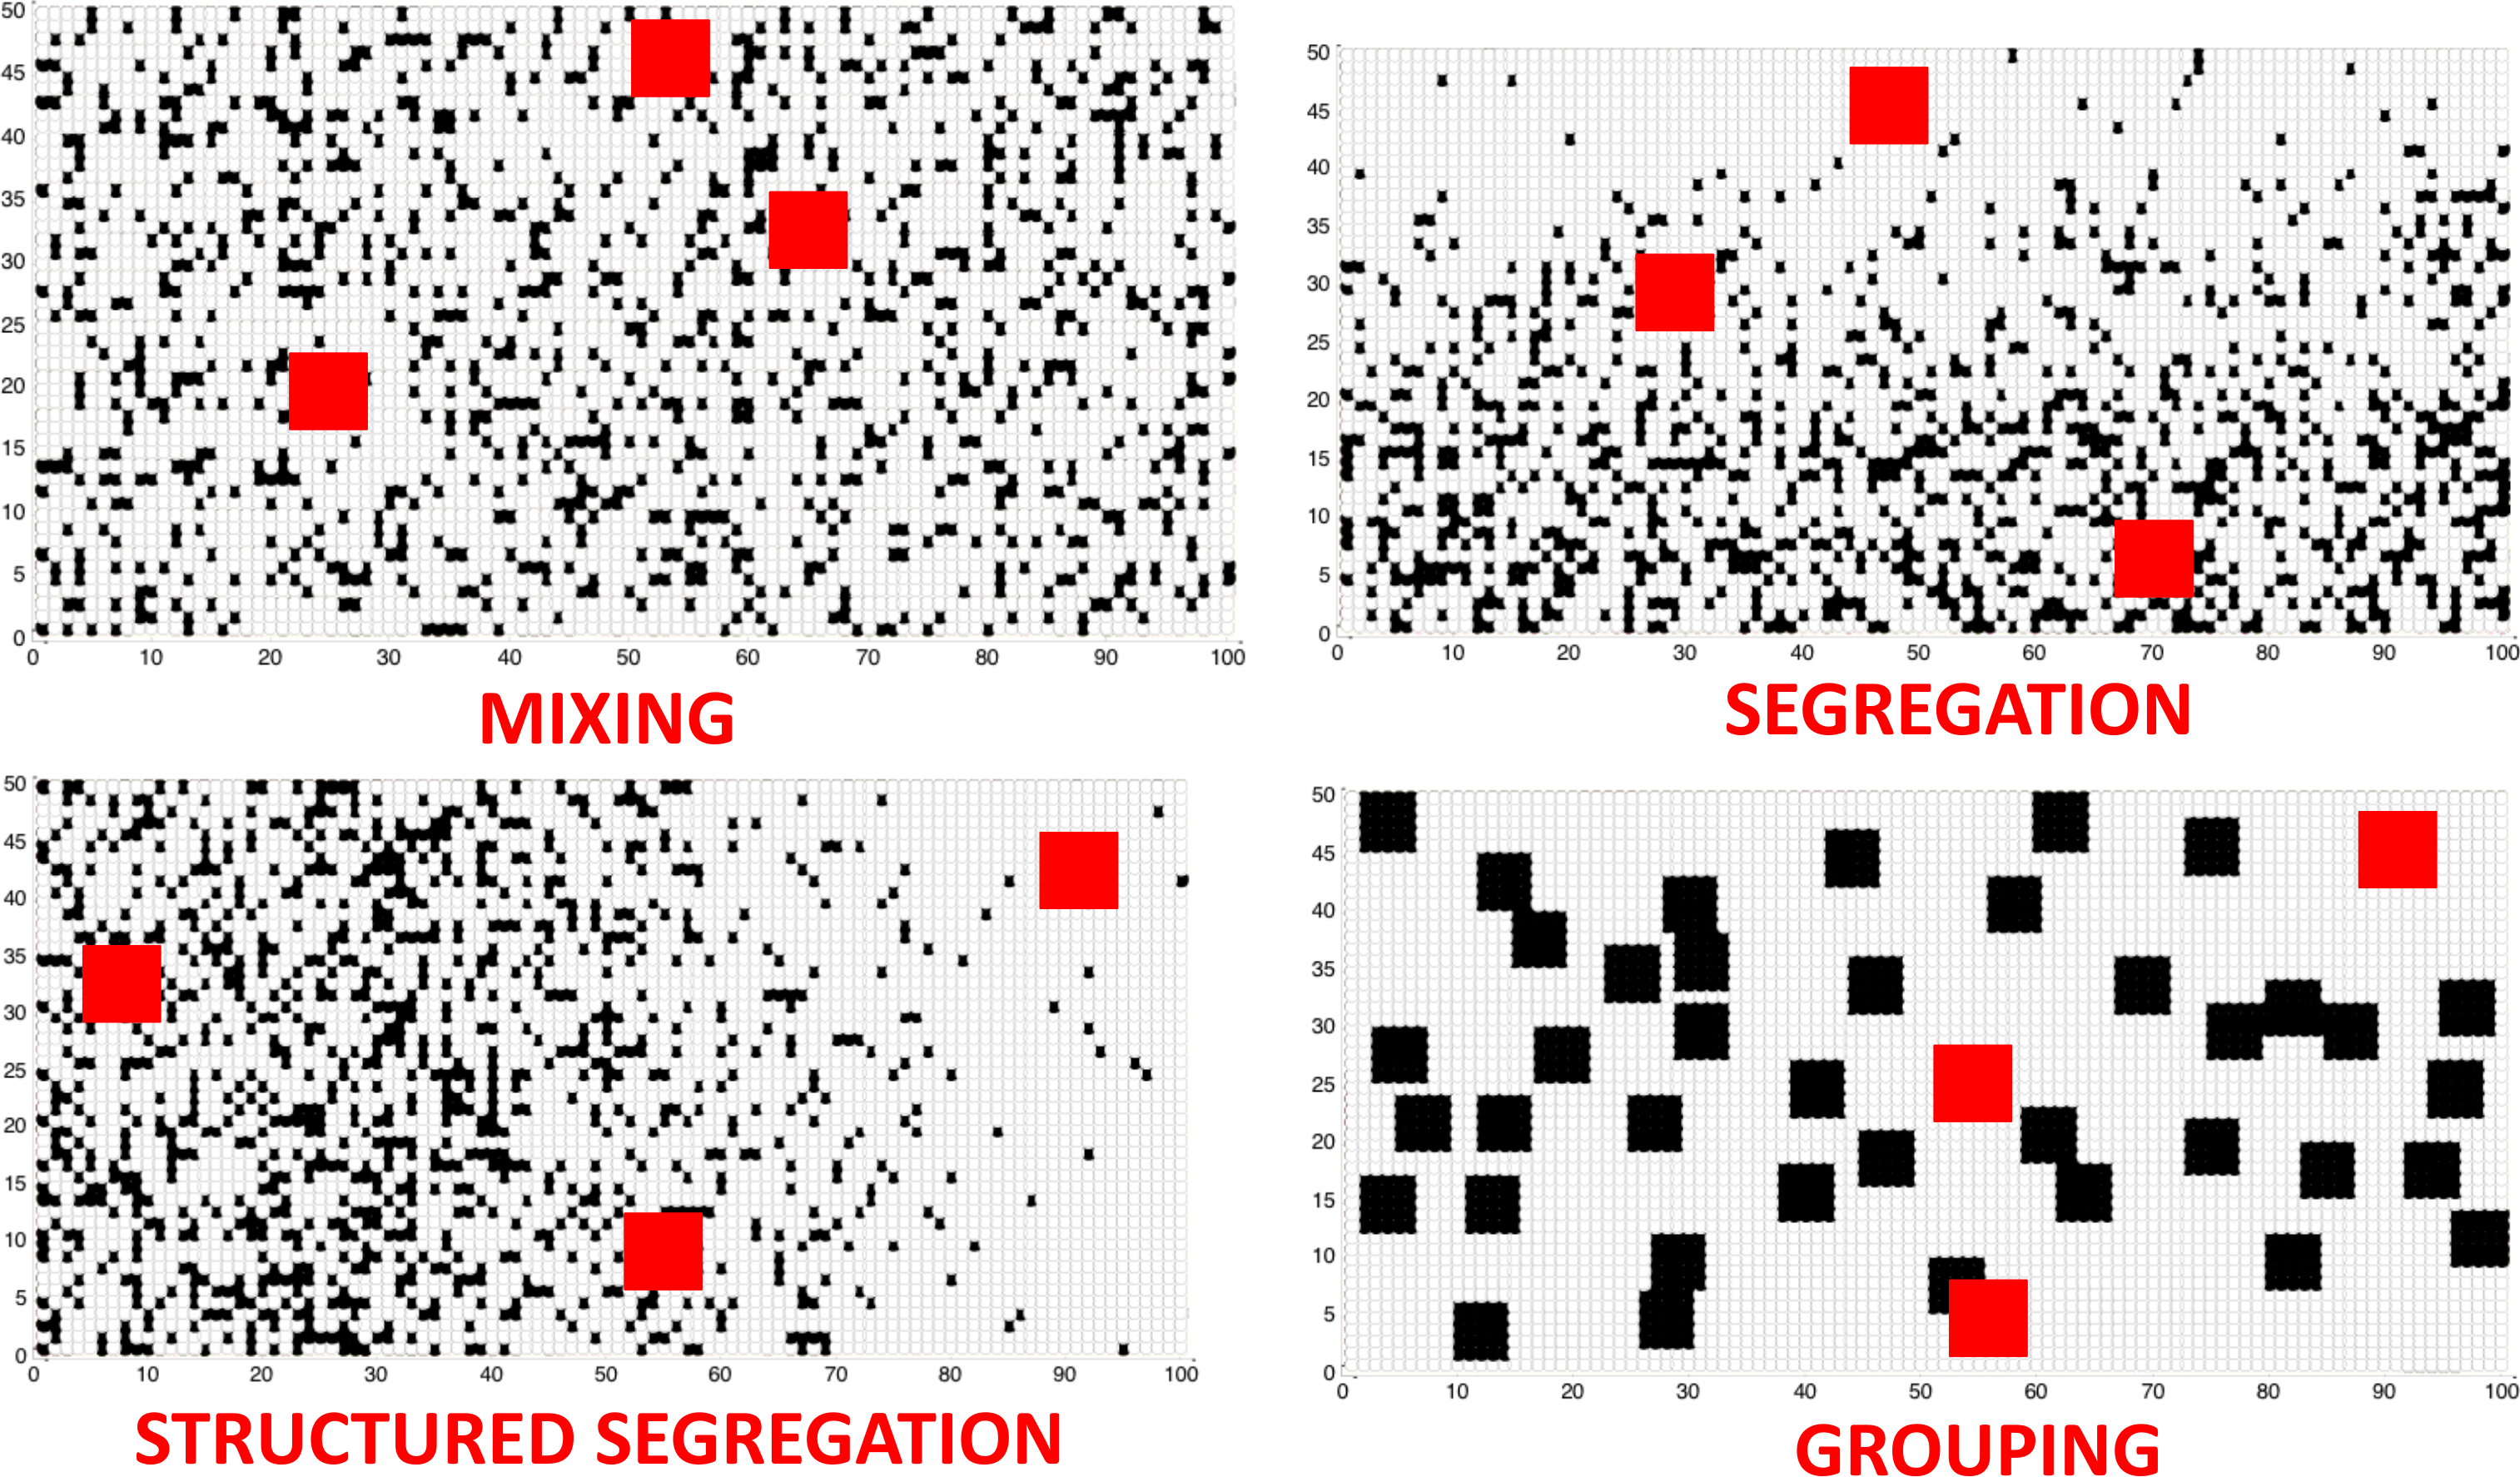
\includegraphics[width=\textwidth]{media/heterogeneity.png}

\subsection{Theory of Sampling (TOS)}
\begin{enumerate}
    \item Fundamental understanding of the concept of: \textbf{Heterogeneity}
    \item Full knowledge about different types of: \textbf{Sampling errors}
    \item Practical understanding of: \textbf{Sampling Unit Operations}
    \item Ability to analyze sampling problems/issues: \textbf{Heterogeneity Characterization}
\end{enumerate}

\subsubsection{Sampling practice}
TOS = 6 General Principles (GPs) + 4 Sampling Unit Operations (SUOs)

\pph{General Principles}
GPs are normally used in design, planning, optimization of new sampling
processes
\begin{itemize}
    \item FSP: Fundamental Sampling Principle
    \item LDT: Lot Dimensionality Transformation
    \item PSC: Sampling Correctness (bias-free sampling)
    \item SSI: Sampling Scale Invariance
    \item PSS: Sampling Simplicity (primary sampling + mass reduction)
    \item LHC: Lot Heterogeneity Characterization
\end{itemize}

\pph{Sampling Unit Operations}
SUOs are used as active steps in the sampling process
(often used several times + in combination)
\begin{itemize}
    \item SUO 1: Composite Sampling
    \item SUO 2: Mixing / Blending
    \item SUO 3: Comminution
    \item SUO 4: Mass Reduction (Sub-sampling)
\end{itemize}

\newpage
\subsection{TOS' basic terms}
\subsubsection{Lot / Sampling Target / Decision Unit}
The complete entity of the original material being subject to sampling e.g. truck load,
process stream, ship’s cargo, bags etc. The lot (sampling target) refers both to the physical,
geometrical form and size, as well as the material characteristics of the material being subject
to sampling.

\paragraph{Dimension of the Lot}
\begin{center}
    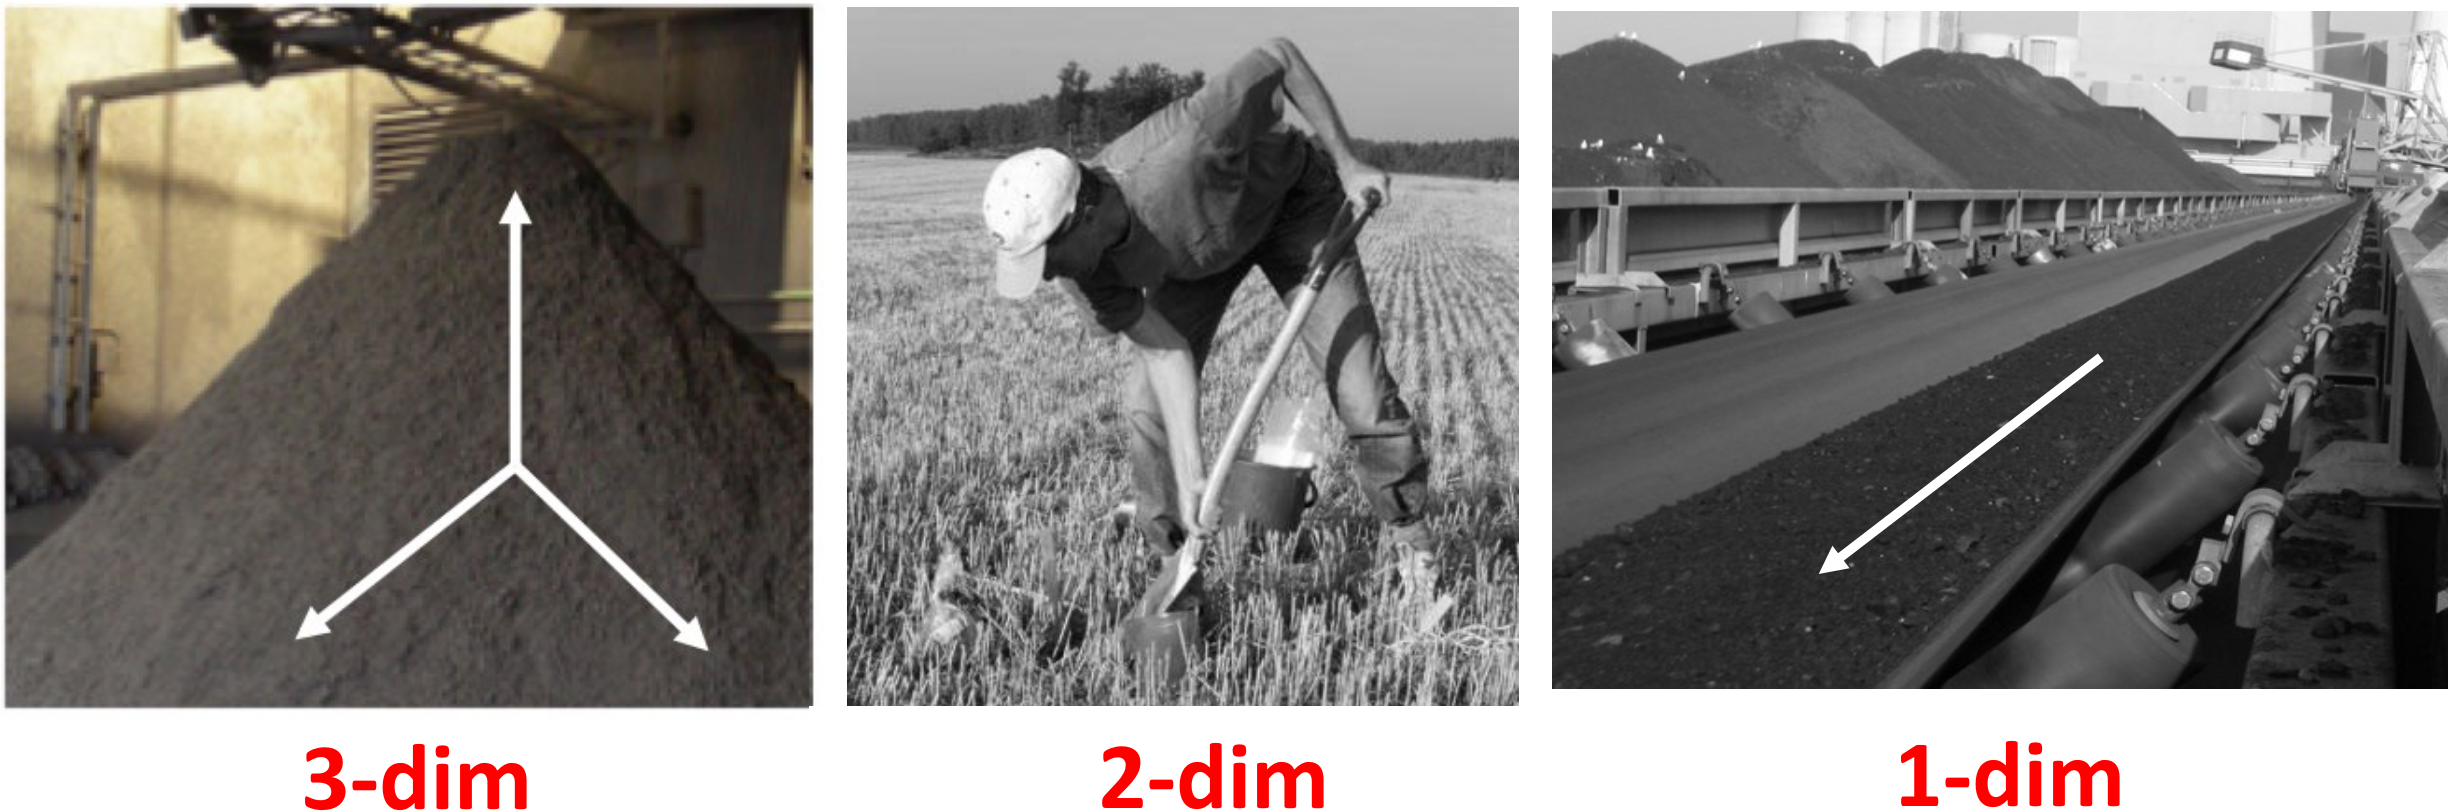
\includegraphics[width=.8\textwidth]{media/dimensions.png}
\end{center}

\pph{Increment}
Correctly delineated and materialized unit of the lot which, combined with other
increments, provides a composite sample.

\pph{Sample}
Correctly extracted material from the lot, which can only originate from a qualified
`correct' sampling process. Composite sample consists of various increments.

\pph{Specimen}
A `sample' that cannot be documented to be representative (because it cannot be
associated with a representative sampling process).

\pph{Fragment}
Fragment refers to the smallest separable unit of the lot
that is not affected by the sampling process itself (e.g.
particles, molecules, grains, etc).

\pph{Group}
A number of spatially correlated fragments, which act as a
coherent unit during sampling operations.

\pph{Representative Sample}
! Sampling bias is not of the same nature as analytical bias !
\begin{itemize}
    \item Must be based on correctly delineated and materialized unit of the lot
    \item Must be based on combination of increments (composite sample)
    \item A sample can only be representative if the sampling process is both accurate (systematic part) and precise / reproducible (random part)
\end{itemize}
\begin{center}
    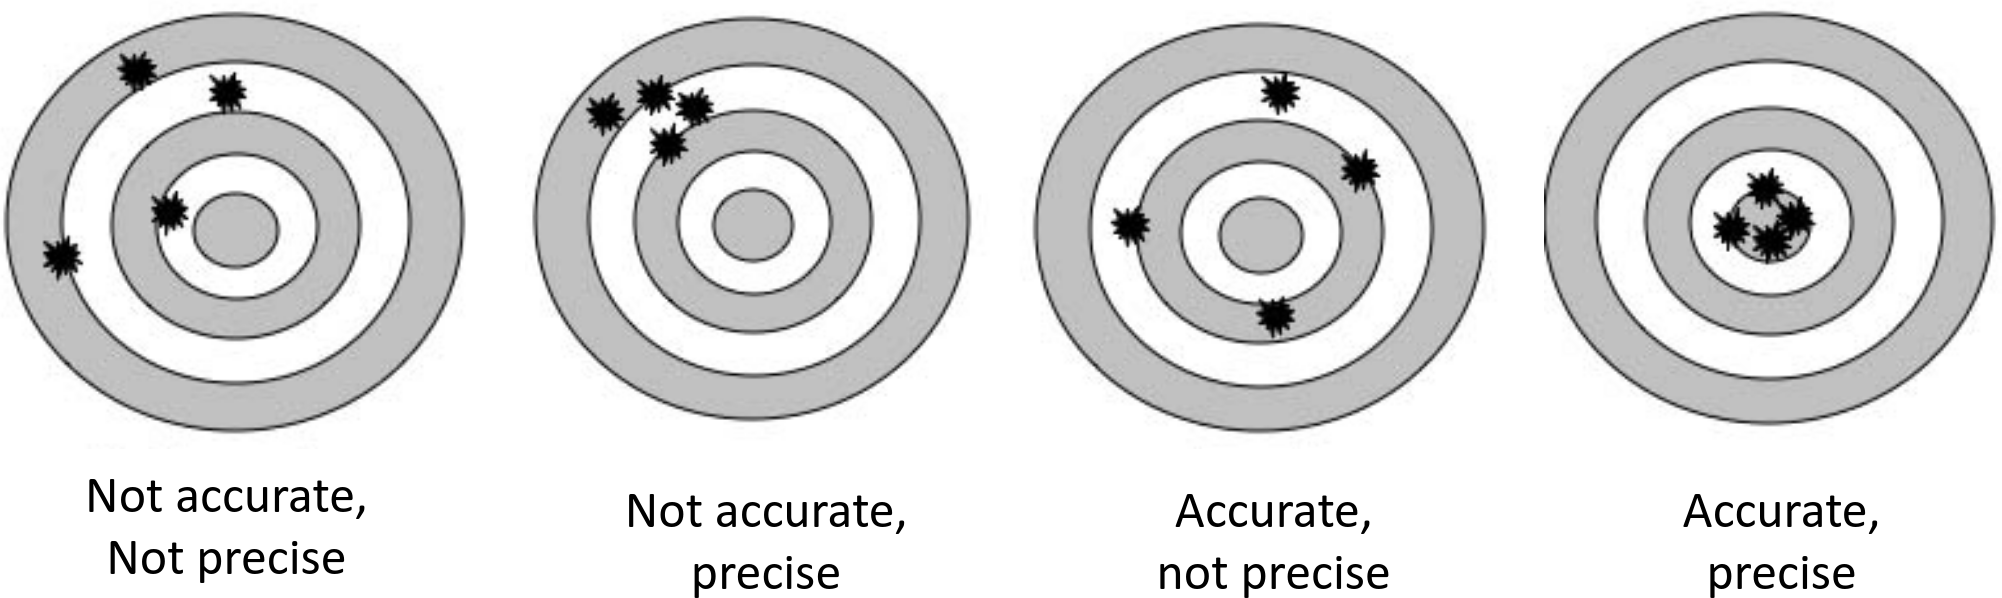
\includegraphics[width=\textwidth]{media/analytical_bias.png}
\end{center}

\pph{Relative sampling error}
\vspace*{-.5cm}
\figbox{$\dm e = \frac{aS-aL}{aL}$}

where:
\begin{itemize}
    \item $aL$ = analytical grade of the lot (grade = mass of analyte divided by the total mass of the lot)
    \item   analytical grade of the sample (mass of analyte divided by the total mass of the sample)
\end{itemize}

\subsection{General Principles (GPs)}
\subsubsection{FSP: Fundamental Sampling Principle}
\begin{itemize}
    \item All possible extractions from the lot (all possible virtual increments) must have the same (non-zero) probability of ending up in the sample
    \item FSP implies physical access to all geometrical units of the lot (access to all the dimensions)
    \item FSP must never be compromised, otherwise possibility of documenting accuracy of the sampling process is impossible
\end{itemize}

\subsubsection{LDT: Lot Dimensionality Transformation}
\begin{minipage}{0.5\textwidth}
    \begin{itemize}
        \item No correlation exist and the increments or fragments can be mixed (any increment can be picked - more or less - freely)\\[1ex]
        \item Increments fully covers two of the lot dimensions (e.g. a ``slice'')\\[1ex]
        \item Increments fully covers one of the lot dimensions (e.g. a drill-core)\\[1ex]
        \item Increments do not fully cover any of the lot dimensions (e.g. a ``stock pile'')
    \end{itemize}
\end{minipage}
\hfill
\begin{minipage}{0.4\textwidth}
    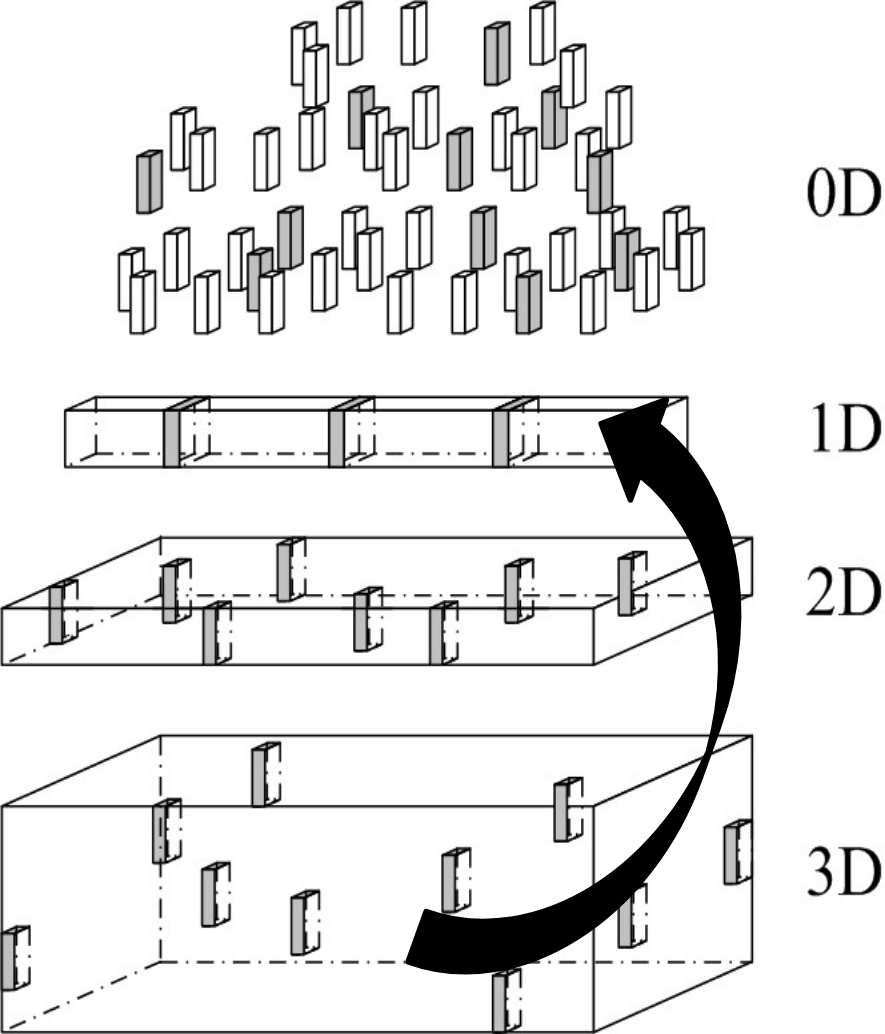
\includegraphics[width=\linewidth]{media/LDT.png}
\end{minipage}

\newpage
\subsubsection{PSC: Principle of Sampling Correctness (bias-free sampling)}
``A sample can only be representative if the sampling process is
both accurate (bias-free) and precise''
\begin{center}
    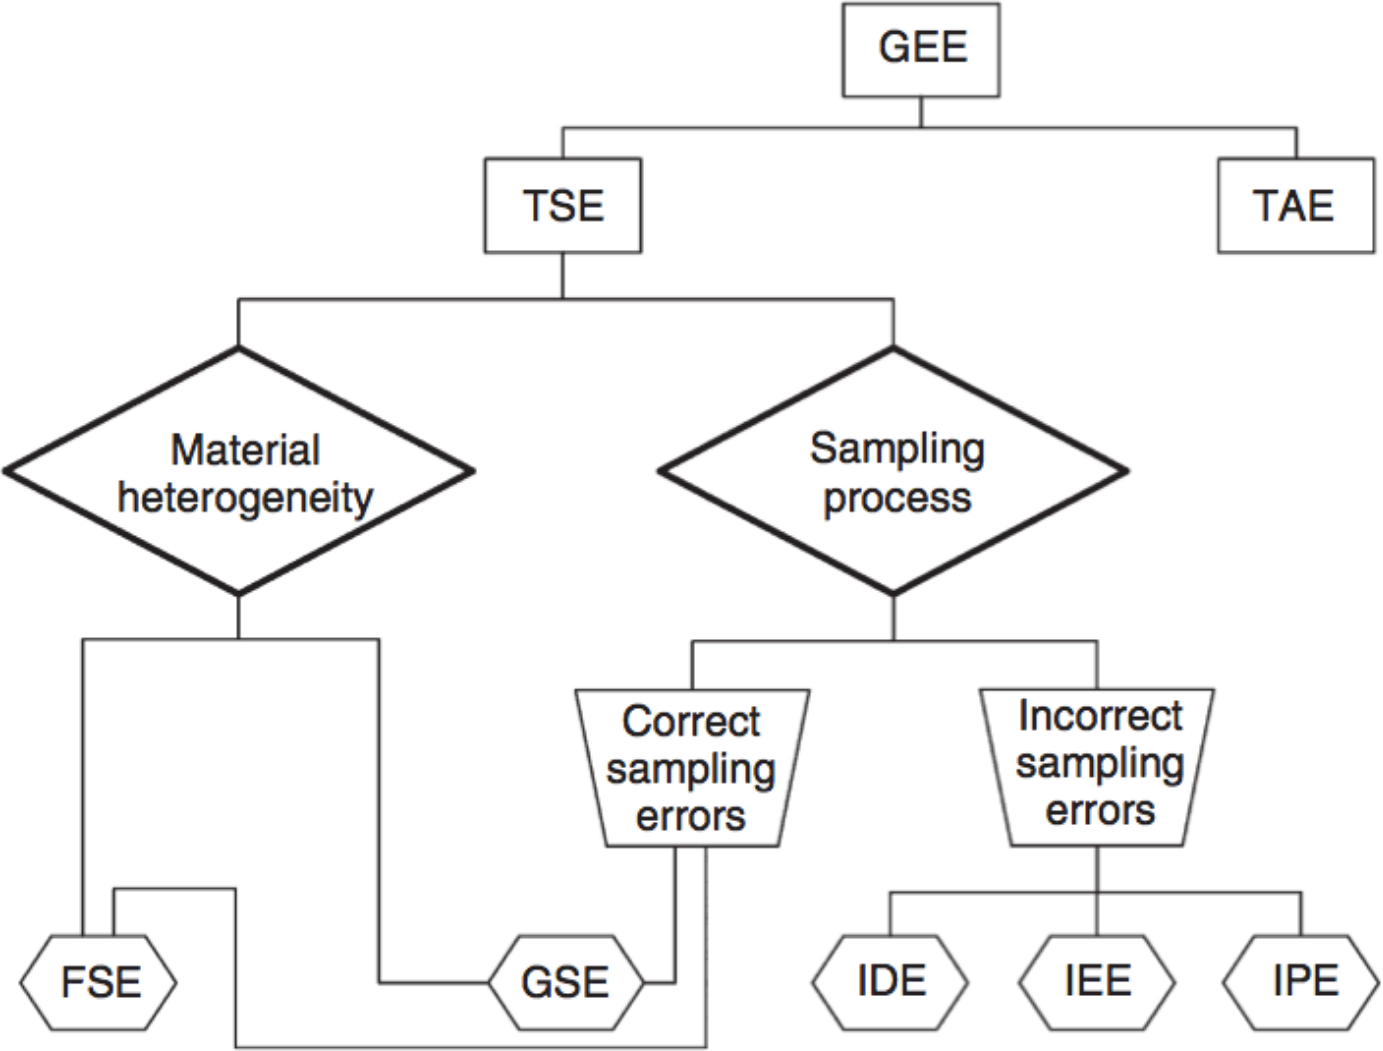
\includegraphics[width=.8\textwidth]{media/PSC.png}
\end{center}

where:
\begin{itemize}
    \item GEE = Global Estimation Error
    \item TSE = Total Sampling Error
    \item TAE = Total Analytical Error
\end{itemize}

\subsubsection{Incorrect sampling errors}
\paragraph{IDE: Increment Delimitation (delineation) Error}
\begin{itemize}
    \item IDE relates to the physical extraction of the increments
    \item IDE can be avoided by delineating an increment which covers the relevant dimensions of the lot
    \item For 1-D lots a correctly delineated increment consists a complete cross-sectional slice of the material stream
\end{itemize}
\begin{center}
    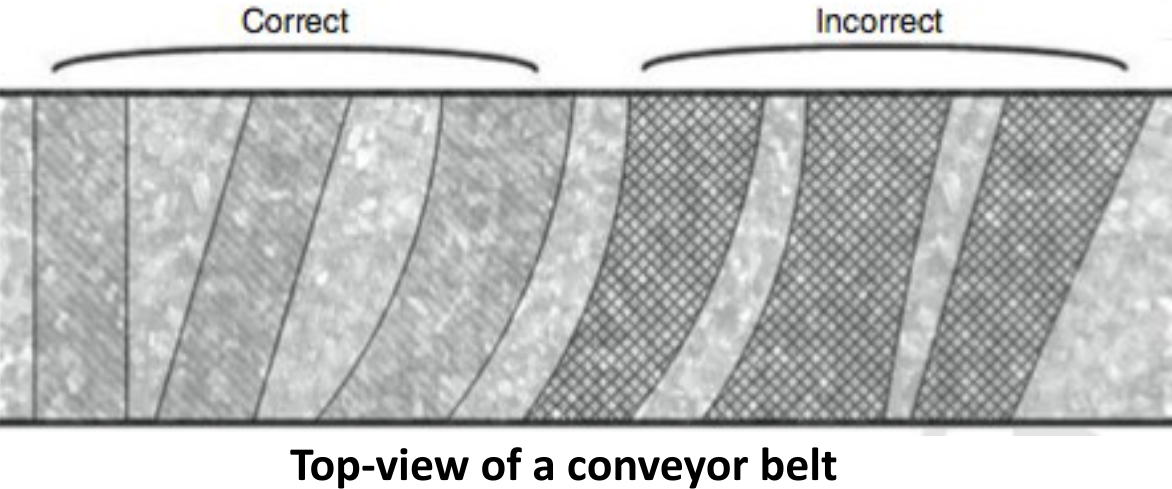
\includegraphics[width=.6\textwidth]{media/IDE.png}
\end{center}

\newpage
\pph{IEE: Increment Extraction Error}
IEE occurs when particles inside the delineated increment do not end up in the sample,
also referred to as the ``centre-of-gravity rule''.
\begin{center}
    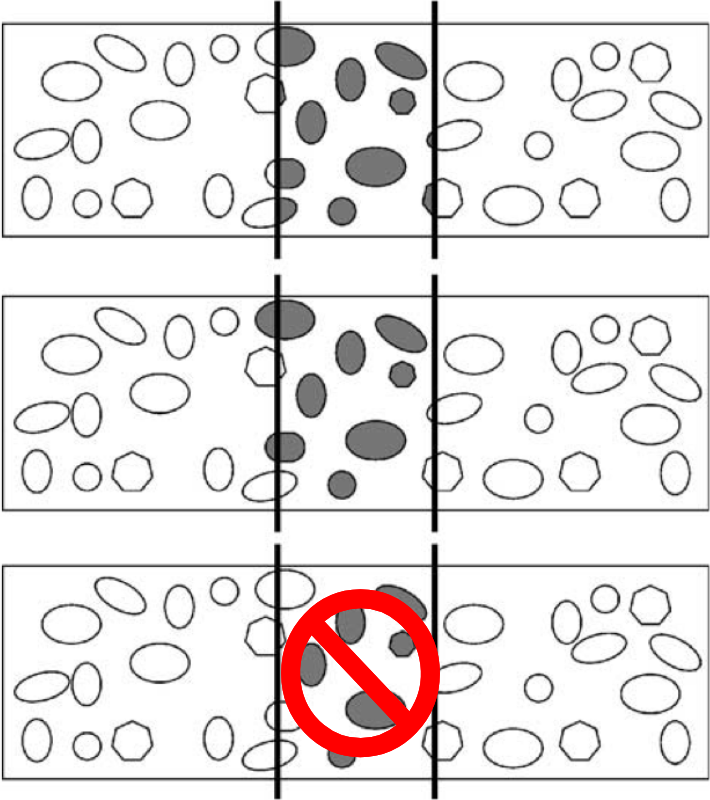
\includegraphics[width=.4\textwidth]{media/IEE.png}
\end{center}

\paragraph{IPE: Increment Preparation Error}
\begin{itemize}
    \item IPE arises when increments/samples are altered after extraction, e.g. contamination, evaporation, moisture absorption, loss of material (spillage), and also deliberate manipulation (fraud, sabotage)
    \item Samples always need to be air-tight sealed, labeled and documented
\end{itemize}

\pph{Sampling process results}
After sample extraction no possibility exists to proof
whether a sample is representative (of the lot) or not.

$\to$\ It must be ensured that the sampling process itself is representative (elimination of all
bias-generating sampling errors)














\end{document}
